\section{平面图形分析}
平面图形分析是制图和三维建模工作中非常重要且很关键的步骤,是准确绘制图样和构建构模型的基础。平面图形分析的目的是分析和了解平面图形中各图形要素之间的相互位置关系,图形之间的依赖关系。图样中的各种尺寸是用于确定图样中图形对象的形状和位置。平面图分析是否准确、是否透彻,直接决定着绘图过程的正确性,也决定着能不能绘制图样和构建模型。

平面图形分析主要是进行平面图形的尺寸分析和平面图形要素的性质分析\footnote{平面图形要素性质分析也称为线段分析} 两个方面的内容。

\subsection{尺寸分析}
平面图形尺寸分析的目的是确定图形元素的尺寸基准、定形尺寸和定位尺寸。尺寸基准、定形尺寸和定位尺寸是平面图形尺寸分析的三大要素。

\begin{figure}[htbp]
\centering
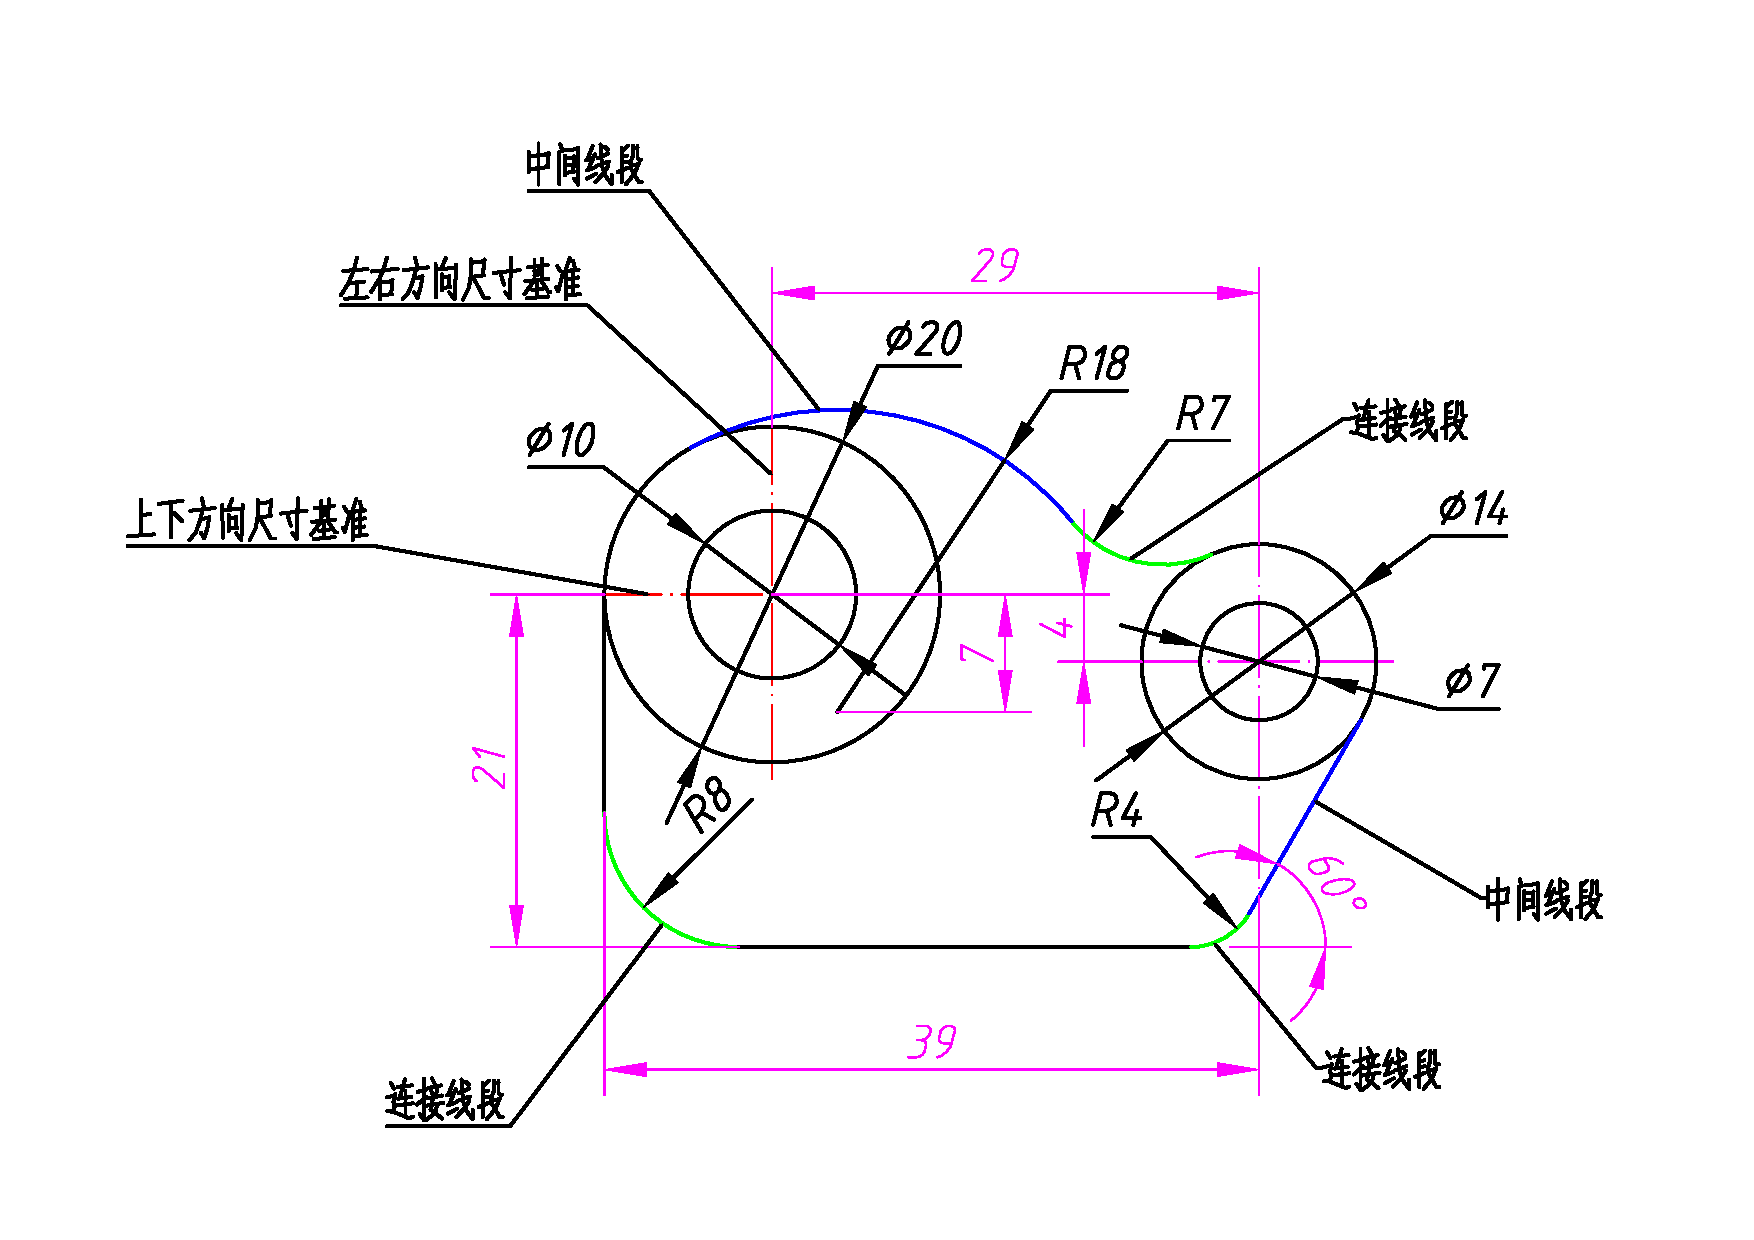
\includegraphics[scale=0.35]{biaozu.pdf}
\caption{平面图形的尺寸和线段分析} \label{fig:biaozu}
\end{figure}

\subsubsection{尺寸基准} 

尺寸基准是绘制和标注尺寸的起点,通常有水平和垂直两个方向的尺寸基准。实际工程图样中常采用图形的对称中心线,较大圆的中心线或主要轮廓线作为尺寸基准线。图\ref{fig:biaozu}所示图形主要是以长度为99mm的轮廓线和$\phi 20$圆的中心线作为垂直方向和水平方向的尺寸基准。

\subsubsection{定形尺寸} 

定形尺寸是确定平面图形中各种线段形状和大小的尺寸,如直线的长度、圆和圆弧的直径或半径、角度的大小等。图\ref{fig:biaozu6}中的$\phi 10$、$\phi 20$、 $\phi 14$、 $R8$、$R18$、$R7$等尺寸均为图\ref{fig:biaozu}的定形尺寸。

\begin{figure}[htbp]
\centering
\begin{floatrow}
\ffigbox{\caption{定形尺寸}\label{fig:biaozu6}}{
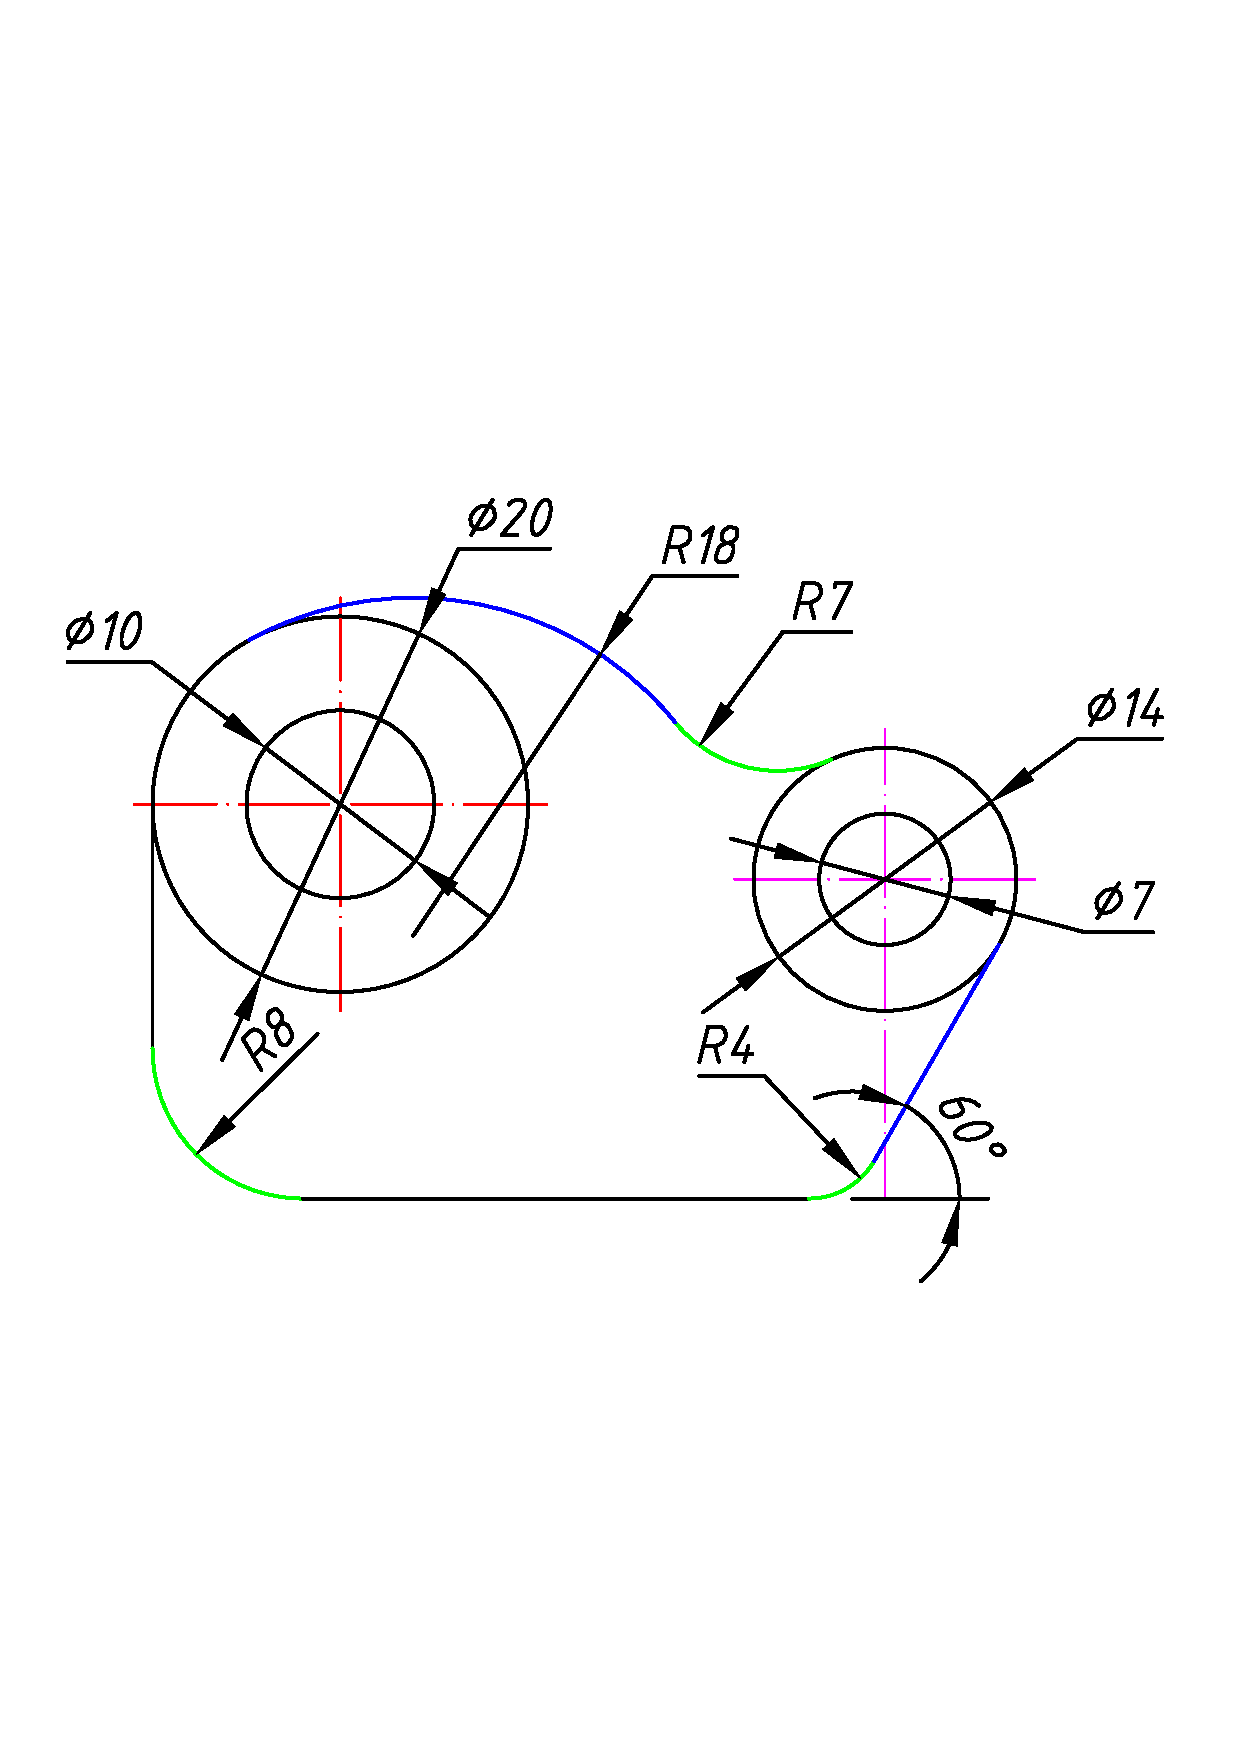
\includegraphics[scale=0.25]{biaozu6.pdf}
}
\ffigbox{\caption{定位尺寸}\label{fig:biaozu5}}{
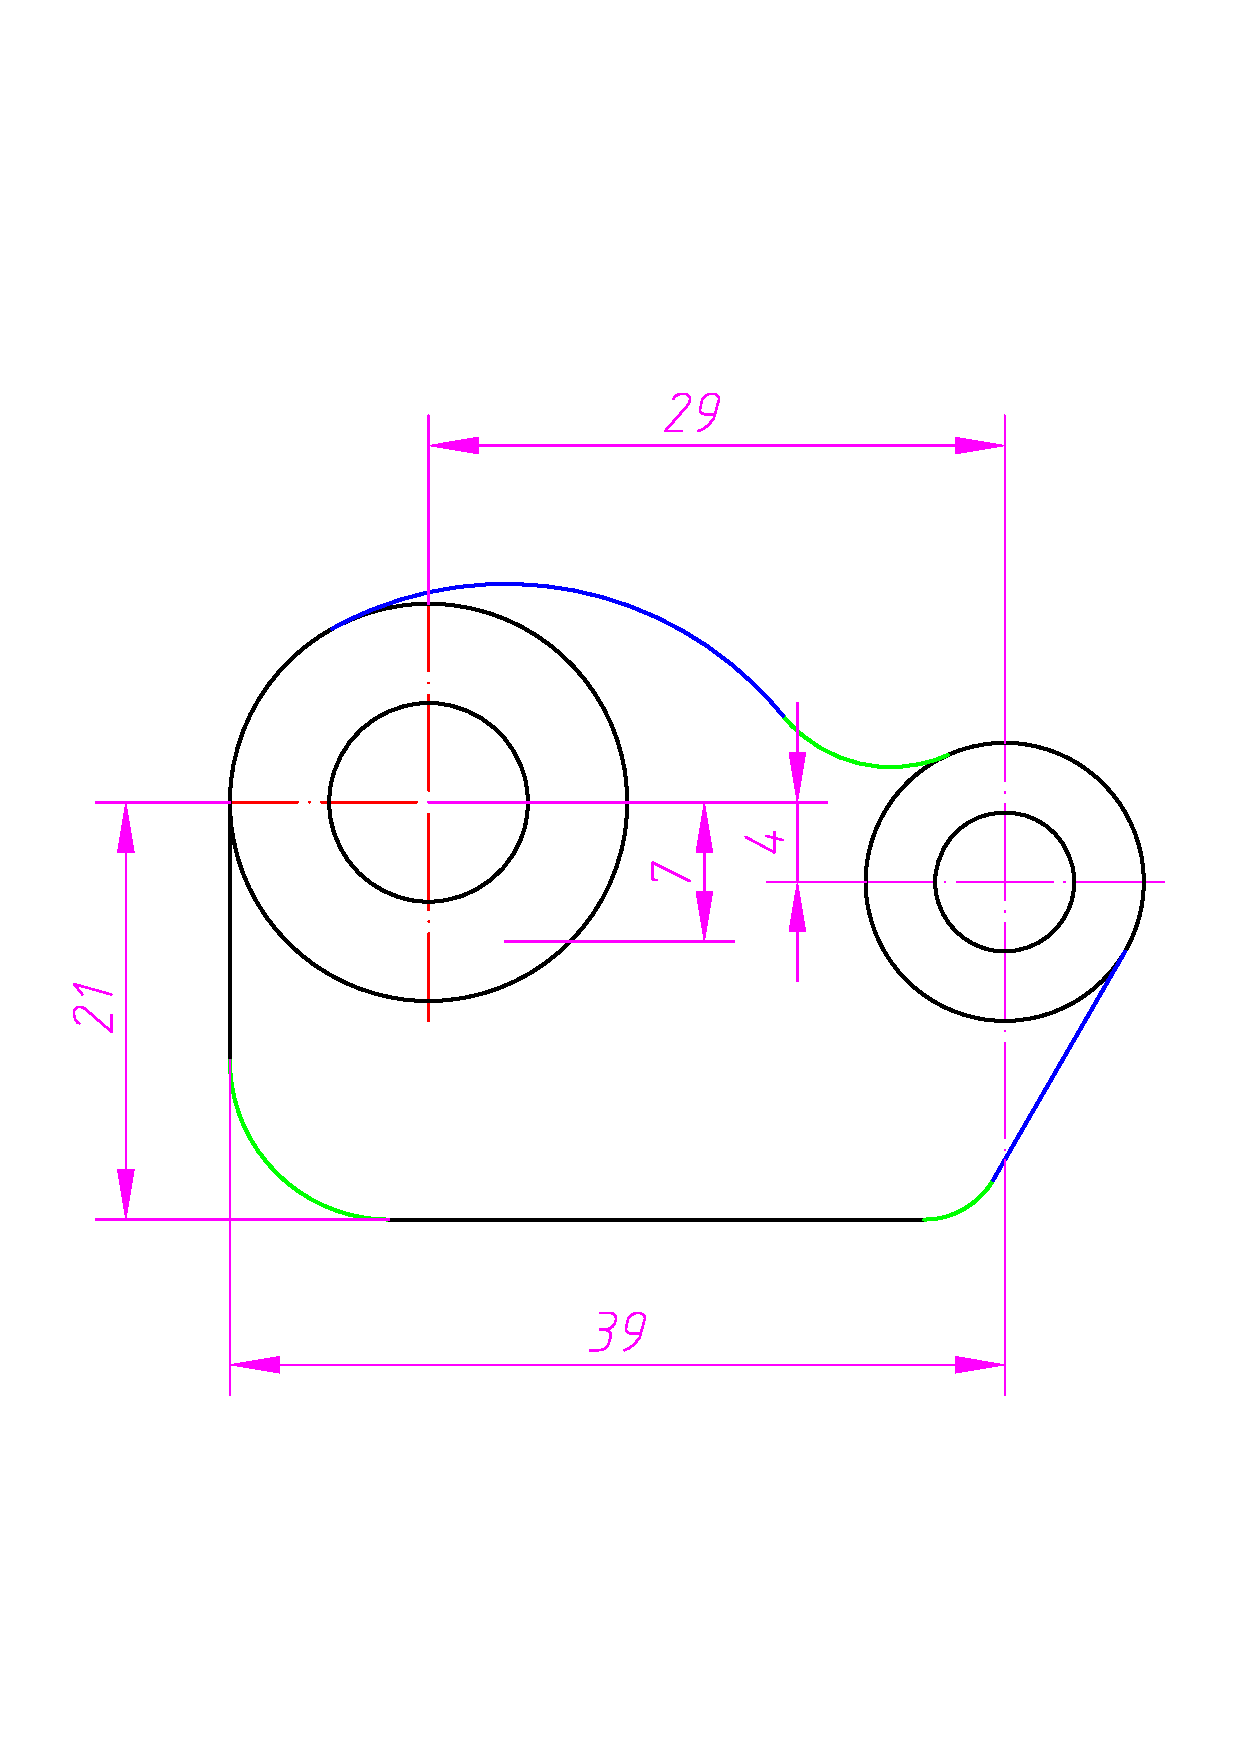
\includegraphics[scale=0.2]{biaozu5.pdf}
}
\end{floatrow}
\end{figure}

\subsubsection{定位尺寸} 

定位尺寸是确定平面图形中各线段之间相对位置的尺寸,图\ref{fig:biaozu5}中标出的尺寸均为图\ref{fig:biaozu}的定位尺寸,其中4和29用于确定$\phi 14$圆的圆心位置。

图\ref{fig:tiaoyafadianpian})中$\phi 104$圆的对称中心线是主视图的尺寸基准,$\phi 53,\phi 104,6-\phi 8$是定形尺寸,$\phi 104$圆的圆心和$\phi 84$为定位尺寸。

\endinput